% ***********************************************************
% ******************* PHYSICS HEADER ************************
% ***********************************************************
% Version 2
\documentclass[11pt]{article} 
\usepackage{amsmath} % AMS Math Package
\usepackage{amsthm} % Theorem Formatting
\usepackage{amssymb}	% Math symbols such as \mathbb
\usepackage{graphicx} % Allows for eps images
\usepackage{multicol} % Allows for multiple columns
\usepackage[dvips,letterpaper,margin=0.75in,bottom=0.5in]{geometry}
 % Sets margins and page size
\pagestyle{empty} % Removes page numbers
\makeatletter % Need for anything that contains an @ command 
\renewcommand{\maketitle} % Redefine maketitle to conserve space
{ \begingroup \vskip 10pt \begin{center} \large {\bf \@title}
	\vskip 10pt \large \@author \hskip 20pt \@date \end{center}
  \vskip 10pt \endgroup \setcounter{footnote}{0} }
\makeatother % End of region containing @ commands
\renewcommand{\labelenumi}{(\alph{enumi})} % Use letters for enumerate
% \DeclareMathOperator{\Sample}{Sample}
\let\vaccent=\v % rename builtin command \v{} to \vaccent{}
\renewcommand{\v}[1]{\ensuremath{\mathbf{#1}}} % for vectors
\newcommand{\gv}[1]{\ensuremath{\mbox{\boldmath$ #1 $}}} 
% for vectors of Greek letters
\newcommand{\uv}[1]{\ensuremath{\mathbf{\hat{#1}}}} % for unit vector
\newcommand{\abs}[1]{\left| #1 \right|} % for absolute value
\newcommand{\avg}[1]{\left< #1 \right>} % for average
\let\underdot=\d % rename builtin command \d{} to \underdot{}
\renewcommand{\d}[2]{\frac{d #1}{d #2}} % for derivatives
\newcommand{\dd}[2]{\frac{d^2 #1}{d #2^2}} % for double derivatives
\newcommand{\pd}[2]{\frac{\partial #1}{\partial #2}} 
% for partial derivatives
\newcommand{\pdd}[2]{\frac{\partial^2 #1}{\partial #2^2}} 
% for double partial derivatives
\newcommand{\pdc}[3]{\left( \frac{\partial #1}{\partial #2}
 \right)_{#3}} % for thermodynamic partial derivatives
\newcommand{\ket}[1]{\left| #1 \right>} % for Dirac bras
\newcommand{\bra}[1]{\left< #1 \right|} % for Dirac kets
\newcommand{\braket}[2]{\left< #1 \vphantom{#2} \right|
 \left. #2 \vphantom{#1} \right>} % for Dirac brackets
\newcommand{\matrixel}[3]{\left< #1 \vphantom{#2#3} \right|
 #2 \left| #3 \vphantom{#1#2} \right>} % for Dirac matrix elements
\newcommand{\grad}[1]{\gv{\nabla} #1} % for gradient
\let\divsymb=\div % rename builtin command \div to \divsymb
\renewcommand{\div}[1]{\gv{\nabla} \cdot #1} % for divergence
\newcommand{\curl}[1]{\gv{\nabla} \times #1} % for curl
\let\baraccent=\= % rename builtin command \= to \baraccent
\renewcommand{\=}[1]{\stackrel{#1}{=}} % for putting numbers above =
\newtheorem{prop}{Proposition}
\newtheorem{thm}{Theorem}[section]
\newtheorem{lem}[thm]{Lemma}
\theoremstyle{definition}
\newtheorem{dfn}{Definition}
\theoremstyle{remark}
\newtheorem*{rmk}{Remark}

% ***********************************************************
% ********************** END HEADER *************************
% ***********************************************************
\usepackage{cancel}
\usepackage{enumerate}
\usepackage{verbatim}
\usepackage{graphicx}
\usepackage{appendix}
\title{Comp 251 Assignment 3}
\author{Ian Benlolo, 260744397 \\ McGill University\\}

\begin{document}
\maketitle
\begin{enumerate}[1.]
%%question 1
\item 
Since we have a tree we could 2 colour it and count how many of every colour we have. 

\begin{verbatim}
algo largestNode(t)
input: A tree t
output: largest number of non adjacent nodes
colour all leaves
mark leaves visited
for i=1 to max(deg(t))
  for all nodes n of degree i
    if neighbours of node n aren't coloured OR n isn't coloured
      colour node n
      mark n visited
    else
      mark n visited
      continue
    endif
  i++
  endfor
endfor
return number of coloured nodes
\end{verbatim}
What the above algorithm is doing is it is starting with the leaves and colouring them. Then checking all nodes with degree 2 and seeing if each has a neighbour or not. If not, it colours them. And it does this until it reaches all the nodes (by increasing the degree and checking every node of every degree this way). \\

%%%question 2
\item
Since we want to maximize the average finishing times of these jobs, we want to have, vulgarly speaking, the most amount of jobs ending as early as possible. \\

Say processing them in increasing order according to their processing times would not minimize the average finishing times of these jobs. Assuming that after ordering them in increasing order we would yield the following ordering $t_1, t_2,\dots, t_n$. After one job, the time that has passed would have been $t_1$. After two jobs, the time passed would have been $t_1+t_2$, and so on. The average times after one job would have been $t_1/1$, after two jobs it would have been $(t_1+t_1+t_2)/2$, and so on.\\
If this weren't the case and the lowest average finishing times for say, only two jobs, would have been yielded with an ordering of $t_2, t_1$, then the average time after the two would have been $(t_2+t_2+t_1)/2$. We have encountered a contradiction because $t_1 < t_2$ therefore $(t_2+t_2+t_1)> (t_1+t_1+t_2)$. QED.


%%question 3
\item
Initially, this problem seems significantly more complicated than the previous one but after contemplating for a little while, it is obvious that it is only an extension of the previous one, and not much more complicated. \\ 
If we look at each processor, $p_1, p_2, p_3$ separately, and analyze the jobs running on it this problem becomes the same as the previous one. We simply want the runtimes of all the jobs on each processor to be ordered in increasing order (proven in $2.$), which can only be accomplished by initially organizing the jobs in increasing order (intuitively). 

%%question 4
\item
I will disprove this using a counterexample. See the following figure:\\
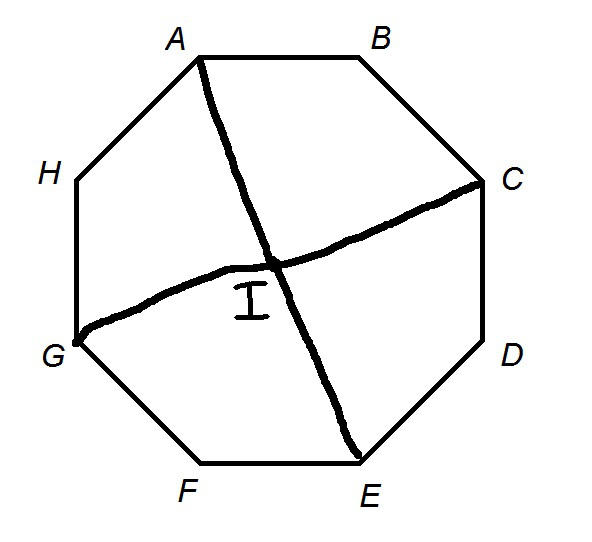
\includegraphics[width=0.4\textwidth]{graph.jpg}\\
If we were to follow the algorithm, we would start with node I, then it would take $4$ steps to get rid of the rest of the edges totalling to $5$ steps but if we were to ignore the algorithm and do this intuitively, this can be done in only $4$ steps starting with A , then C, E and finally G. 


%%question 5
\item
\begin{verbatim}
Algo smallestCircle(double x[], double y[])
input: two arrays (of size n) corresponding to coordinates on an x-y plane
output (x,y)-value and radius of circle

distanceToCircle[n]
for i=0 to n
   point p=(x[i],y[i])
   distanceToPoint[n];
   for j=0 to n
      point p2=( x[j],y[j] )
      distanceToPoint[j]=distance( p, p2 )
   end for
   point x=findMedian(distanceToPoint) //maybe sort it using mergesort and take middle point
   distanceToCircle[i]=x
end for
d=findSmallest(distanceToCircle);
findIndex(d, distanceToCircle)
return x[i], y[i], d
\end{verbatim}

What I did is iterate through each point and at each iteration find the distance from it to every other point. I then found the median of this (which would correspond to the smallest radius containing half of the points) and stored it in an array. This array now contains the smallest radius containing at least half the point for every point. From here I just found the smallest of this and returned that value and the $x, y$ values corresponding to the centre point. 

%%question 6
\item
We start with the tree $T=F$. At every iteration of our algorithm we add the lowest cost edge the $G$ excluding $F$ which does not produce a cycle in T. Continue until T has $n-1$ edges or we have gone through all the edges in $E$, where the algorithm would then return false because that would mean the graph is disconnected. Otherwise it would return the tree $T$. \\
Proving this is quite similar to proving Kruskal's algorithm' proof.\\ Consider any point of this algorithm where it is considering adding node $f$. At this point all the nodes added so far are either $(i)$ cheaper than e, or $(ii)$ included in F.\\
In $(i), f$ cannot be in the spanning tree with minimum cost which includes $F$ by the cycle property.  Also, $f$ cannot be swapped for an element of $F$ because it must be included, by the original condition imposed by the question. The only reason the algorithm would skip node $f$ is if it created a cycle in $T$.\\We have now successfully proven that $T$ consists of a spanning tree of $G$ with minimal cost and all edges excluded cannot belong to it's spanning tree. 
\end{enumerate}
\end{document}